\documentclass{bachelor_report}

% Додаткові пакети вносіть у цей файл
\input{01_packages}
\addbibresource{../BIB/Resources.bib}

% Додаткові визначення та перевизначення команд вносіть у цей файл
\input{02_redefinitions}

% Відомості про автора роботи
\input{03_data}

% Починаємо верстку документа
\begin{document}

\setfontsize{14}

% Створюємо титульну сторінку
\input{../CHAPTERS/a1_title}

%% Створюємо зміст    % -- розкоментуйте, якщо зміст вам потрібен
%\pagenumbering{gobble}
\tableofcontents
\cleardoublepage
%\pagenumbering{arabic}

\setcounter{page}{2}    %!!! -- продумати, як автоматизувати номер сторінки

%% Якщо ви використовуєте зміст, то прослідкуйте, щоб номер сторінки 
%% співпадав із справжнім!

% Створюємо перелік умовних позначень, скорочень і термінів
% Якщо цей розділ вам не потрібен, просто закоментуйте два наступних рядка
%\shortings
%\input{../CHAPTERS/a2_shortings}

% Створюємо вступ
%\intro
\input{../CHAPTERS/a3_introduction}

% Додаємо глави
% Якщо ваша робота містить менше або більше глав - модифікуйте наступні 
% рядки відповідним чином
\input{../CHAPTERS/c1_chapter_01}
% \input{../CHAPTERS/c2_chapter_02}
\section{C\#}

C\# — це сучасна об’єктно-орієнтована мова програмування загального призначення, розроблена корпорацією Microsoft у рамках її ініціативи .NET і пізніше затверджена як стандарт Європейською асоціацією виробників комп’ютерів (ECMA) і міжнародними стандартами (ISO). В основному C\# використовується для розробки Web додатків, ігор та застосунків для Windows. Розгляньмо деякі із бібілотек.

\subsection{Використання GNU GMP бібліотеки із мовою програмування С\#}

Як вже було згадано вище, GNU GMP допомагає виконувати будь які арифметичні операції із довільною точністю, що обмежена лише пам'яттю машини, на якій виконується программа. Для того, щоб використовувати цю бібліотеку в мові програмування СSharp слід встановити до проєкту Nuget пакет із назвою "Math.Gmp.Native.NET".

Бібліотека "Math.Gmp.Native.NET" автоматично завантажує на виконання 32-бітну або 64-бітну бібліотеку GNU MP, яка відповідає поточній архітектурі центрального процесора, тим самим дозволяючи будувати проекти Visual Studio для режимів Any CPU, x86 або x64. Вона базується на розширеній збірці GNU MP, яка автоматично визначає тип поточного процесора і вибирає оптимізацію коду на мові асемблера для даного процесора, тим самим забезпечуючи найкращу продуктивність. 

Клас Math.Gmp.Native.gmp\_lib містить статичний метод для кожної з функцій GNU MP. Інші типи визначені для відтворення структур і псевдонімів типів GNU MP і мов C, а також мовних конструкцій C.

Заради зручності цю довідку було створено з офіційного посібника GNU MP версії 6.1.2. Вона демонструє, з прикладами, як кожна функція GNU MP викликається в .NET.

Для початку порівняємо код мовою програмування C\# із кодом на Rust.(рис. 1)

\begin{figure}[!h]
     \centering
     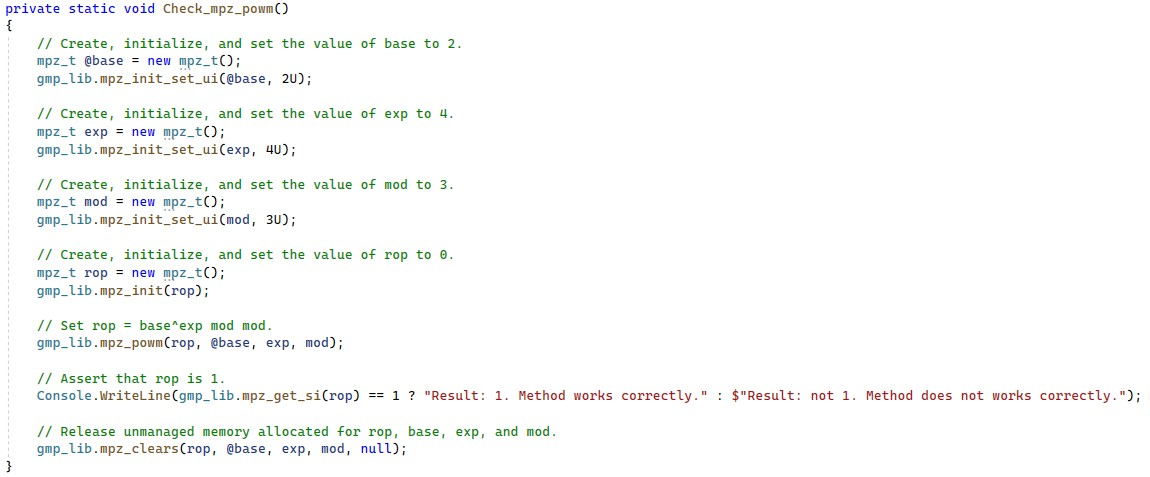
\includegraphics[scale = 1]{../IMAGES/image_01_c_sharp_lab_01.jpg}
     \caption{Приклад піднесення до степеня.}
     \label{fig:}
\end{figure}

Видно, що для використання GMP треба використати змінні класу mpz\_t і задавати певні значення чисел у функцію mpz\_pown. Якщо метод відпрацював успішно, то в консолі можна буде побачити повідомлення про коректну роботу. (рис. 2)

\begin{figure}[!h]
     \centering
     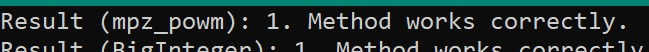
\includegraphics[scale = 1]{../IMAGES/image_02_c_sharp_lab_02.jpg}
     \caption{Приклад для перевірки коректності роботи алгоритму.}
     \label{fig:}
\end{figure}

Розглянемо для остаточного розуміння, як саме використовувати написану мовою програмування C бібліотеку у поєднанні із СSharp оболонкою для знаходження зворотнього елементу. (рис. 3)

\begin{figure}[!h]
     \centering
     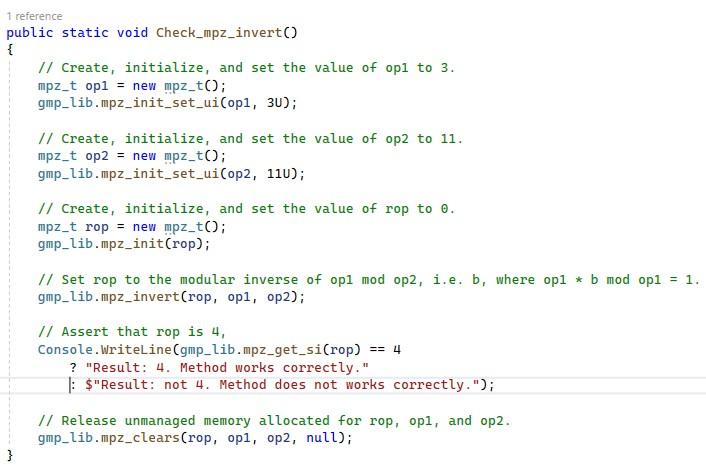
\includegraphics[scale = 1]{../IMAGES/image_05_c_sharp_lab_05.jpg}
     \caption{Приклад знаходження зворотнього елементу.}
     \label{fig_05:}
\end{figure}

\newpage
\par

\subsection{Використання System.Numerics.BigInteger бібліотеки із мовою програмування C\#}

BigInteger - це тип даних в програмуванні, який дозволяє представляти та виконувати операції з великими цілими числами, які виходять за межі можливостей стандартних числових типів. В інших мовах програмування цей тип може мати різні назви, але концепція залишається однаковою - він дозволяє працювати з числами довільної довжини і не обмежується розміром пам'яті, яку може займати число.

У .NET BigInteger знаходиться в просторі імен System.Numerics і забезпечує можливість виконувати арифметичні операції, порівнювати та взаємодіяти з великими цілими числами, незалежно від їх розміру, забезпечуючи точність та надійність операцій. Це особливо корисно при виконанні обчислень, де великі числа можуть виникати при розв'язанні математичних задач, криптографії, обробці великих даних тощо.

Таким чином, маємо реалізацію піднесення до степеню, використовуючи System.Numerics.BigInteger.ModPow.

\begin{figure}[!h]
     \centering
     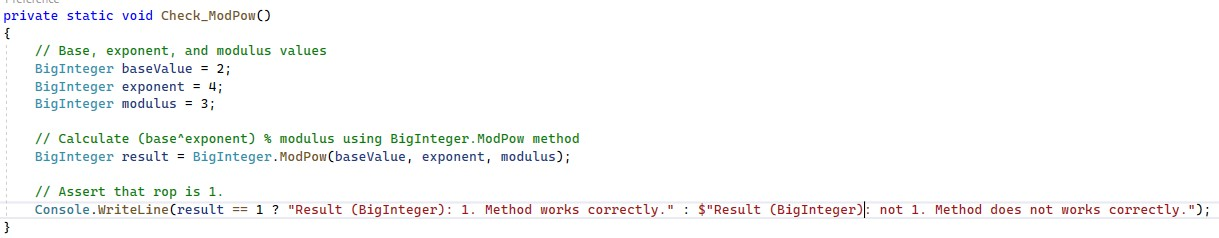
\includegraphics[scale = 1]{../IMAGES/image_03_c_sharp_lab_03.jpg}
     \caption{Приклад піднесення до степеня BigInteger.}
     \label{fig_03:}
\end{figure}

Після виконання такого шматочку коду в результаті побачимо

\begin{figure}[!h]
     \centering
     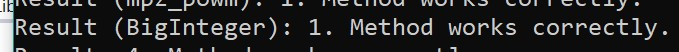
\includegraphics[scale = 1]{../IMAGES/image_04_c_sharp_lab_04.jpg}
     \caption{Результат піднесення до степеня BigInteger.}
     \label{fig_04:}
\end{figure}

Таким чином, бачимо, що обидві функції коректно працюють.


\subsection{Висновки до розділу C\#}

Мова програмування C\# є відмінним вибором для роботи із різними арифметичними операціями, оскільки вона підтримує різні бібліотеки для роботи з великими числами та арифметикою високої точності. Перш за все, вбудований клас System.Numerics.BigInteger надає можливість оперувати дуже великими цілими числами без втрати точності, що робить його ідеальним вибором для обчислень, де великі числа важливі.

Додатково, наявність зовнішніх бібліотек, таких як Math.Gmp.Native або System.Numerics.MPFR, розширює можливості C\#. Ці бібліотеки забезпечують швидку та ефективну роботу з великими числами, що особливо корисно для вимогливих до продуктивності застосувань. Наприклад, вони можуть бути використані в задачах криптографії, математичних моделях або статистичних розрахунках, де точність та продуктивність є ключовими.

Крім того, можливість використання різних бібліотек дає можливість вибору відповідно до конкретних потреб проекту. Наприклад, System.Numerics.BigInteger надає зручний та простий інтерфейс для роботи з великими числами, тоді як Math.Gmp.Native або System.Numerics.MPFR можуть бути використані для оптимізації продуктивності у вимірюваних додатках.

Загалом, здатність C\# підтримувати і вбудовані, і сторонні бібліотеки для роботи з арифметичними операціями робить її потужним і гнучким інструментом для вирішення широкого спектру математичних завдань у сучасному програмуванні.




\section{Java}

Java -- високорівнева, об'єктно орієнтована мова прогармування, що має на меті дозволити розробникам писати один раз і запускати програми будь-де. Це означає, що скомпільований код Java може працювати на всіх платформах, які підтримують Java, без необхідності повторної компіляції. Розгляньмо бібліотеки і для цієї мови.

\subsection{Використання бібліотеки BigInteger у мові програмування Java}

В мови програмування Java є декілька бібліотек, які можуть працювати з багаторозрядною арифметикою:
\begin{itemize}
    \item \texttt{BigInteger та BigDecimal}. Ці класи є вбудованими в Java і дозволяють вам працювати з цілими числами та десятковими числами великої точності. Вони підтримують арифметичні операції з великою точністю.
    \item \texttt{Apfloat}. Ця Java бібліотека надає інструменти для роботи з десятковою арифметикою з довільною точністю. Вона може бути використана для виконання обчислень з високою точністю, схожих на MPFR.
    \item \texttt{JScience}. Ця бібліотека має підтримку для роботи з великими цілими числами, десятковою арифметикою та багатою функціональністю для числових обчислень.
    \item \texttt{Apache Commons Math}. Ця бібліотека містить різноманітні математичні функції та алгоритми для Java. Вона також містить класи для роботи з десятковою арифметикою та раціональними числами.
\end{itemize}

Але ми зупинимось на вбудованій і достатьньо багатій бібліотеці для роботи з багаторозрядною арифметикою -- \texttt{BigInteger}.

\textbf{BigInteger} -- це потужний інструмент для виконання будь-яких арифметичних операцій з довільною точністю, і його обмеження обумовлене лише ресурсами пам'яті вашої системи.

Бібліотека \texttt{BigInteger} є частиною стандартної бібліотеки Java і входить в пакет \texttt{java.math}. Вам не потрібно встановлювати його додатково, він доступний за замовчуванням при використанні будь-якого стандартного дистрибутива Java. Ви можете імпортувати даний пакет та використовувати для роботи з великими цілими числами у своїх Java програмах без будь-яких додаткових дій.

BigInteger надає аналоги всім примітивним цілочисельним операторам Java та всім відповідним методам із \texttt{java.lang.Math}. Крім того, BigInteger надає операції для модульної арифметики, обчислення GCD, перевірки простоти, генерації простих значень, обробки бітів і кількох інших різних операцій.
Семантика арифметичних операцій точно імітує цілочисельні арифметичні оператори Java. Семантика порозрядних логічних операцій точно імітує побітові цілочисельні оператори Java. Також надаються модульні арифметичні операції для обчислення залишків, піднесення до степеня та обчислення мультиплікативних обернених. Ці методи завжди повертають невід’ємний результат від 0 до (modulus - 1) включно.

BigInteger має $3$ основних поля:
\begin{itemize}
    \item \texttt{static BigInteger	ONE} // Константа BigInteger.
    \item \texttt{static BigInteger	TEN} // Константа BigInteger десять.
    \item \texttt{static BigInteger	ZERO} // Константа BigInteger нуль.
\end{itemize}

Тепер розглянемо декілька методів, які нас цікавлять.

\uline{Метод \textbf{java.math.BigInteger.pow(int exponent)}} використовується для обчислення збільшення BigInteger до степеня деякого іншого числа, переданого як експонента, значення якого дорівнює ($this^{exponent}$). Цей метод виконує операцію над поточним BigInteger, за допомогою якого цей метод викликається, а експонента передається як параметр.

\texttt{public BigInteger pow(int exponent)}

Повертає велике ціле число, значення якого дорівнює ($this^{exponent}$). Зауважимо, що експонента є цілим числом, а не BigInteger.

\uline{Параметри:} \textit{exponent} – експонента, до якої має бути піднесено це $BigInteger$.

\uline{Повернення:} $this^{exponent}$

\uline{Виняток:} \textit{ArithmeticException} – експонента від’ємна. (Це призведе до того, що операція дасть неціле значення.)

\vspace{10pt}
\uline{Приклад використання методу \textbf{BigInteger.pow(int exponent)}:}
\begin{figure}[h]
     \centering
     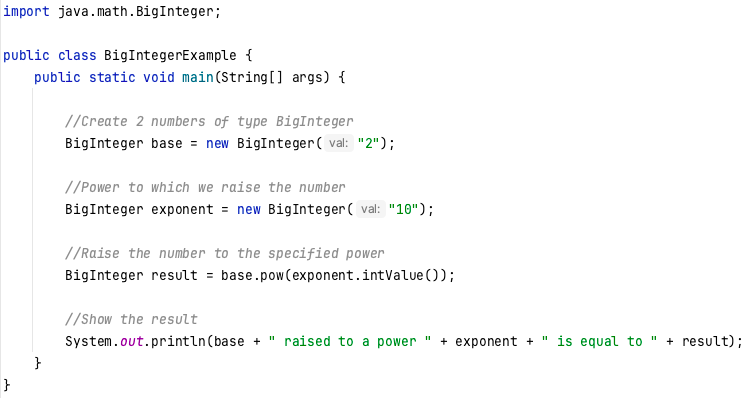
\includegraphics[scale = 0.4]{../IMAGES/Java/BigInt_ex.png}
     \caption{Приклад піднесення до степеня BigInteger.}
     \label{fig_java_pow1}
\end{figure}

\begin{figure}[h]
     \centering
     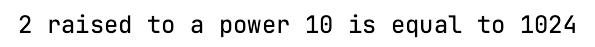
\includegraphics[scale = 0.4]{../IMAGES/Java/BigInt_ex_output.png}
     \caption{Результат піднесення до степеня BigInteger.}
     \label{fig_java_pow2}
\end{figure}

\begin{figure}[h]
     \centering
     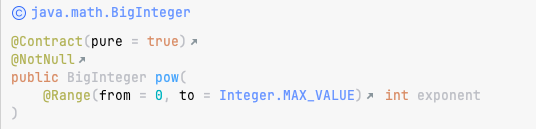
\includegraphics[scale = 0.5]{../IMAGES/Java/BigInt_ex_doc.png}
     \caption{Функція, яка використовується при піднесенні до степеня.}
     \label{fig_java_pow3}
\end{figure}

\newpage
\uline{Метод \textbf{Java.math.BigInteger.modPow()}} повертає BigInteger, значення якого дорівнює ($this^{exponent}$ \textit{mod m)}. Якщо експонента == 1, повертається значення (це mod m), а якщо експонента < 0, повертається модульне мультиплікативне значення (this-exponent). Метод видає ArithmeticException, якщо m <= 0.

\texttt{public BigInteger modPow(BigInteger exponent, BigInteger m)}

\uline{Параметри:} метод приймає два параметри: параметр експоненти, параметр модуля.

\uline{Повернення:} метод повертає об’єкт BigInteger, значення якого дорівнює ($this^{exponent}$\textit{mod m)}.

\uline{Виняток:} \textit{ArithmeticException:} Якщо ($m <= 0$) або експонента від’ємна, і це велике ціле число не є взаємно простим до m.

\uline{Приклад використання методу \textbf{BigInteger.modPow()}:}

\begin{figure}[h]
     \centering
     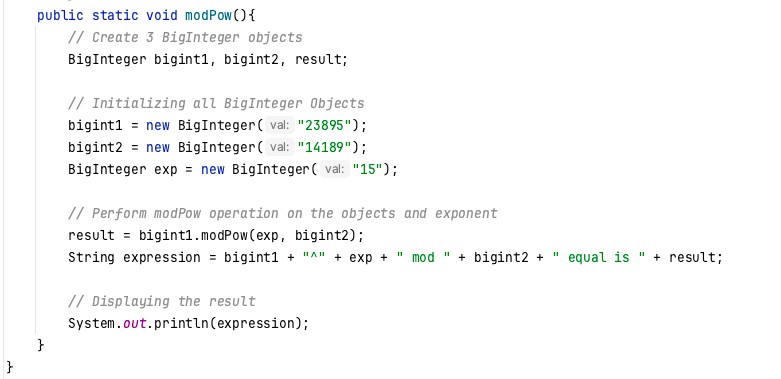
\includegraphics[scale = 0.6]{../IMAGES/Java/BigInt_modPow_ex.png}
     \caption{Приклад піднесення до степеня BigInteger за mod.}
     \label{fig_java_mPow1}
\end{figure}

\begin{figure}[h]
     \centering
     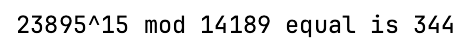
\includegraphics[scale = 0.5]{../IMAGES/Java/BigInt_modPow_output.png}
     \caption{Результат піднесення до степеня BigInteger за mod.}
     \label{fig_java_mPow2}
\end{figure}
\vspace{10pt}
\begin{figure}[h]
     \centering
     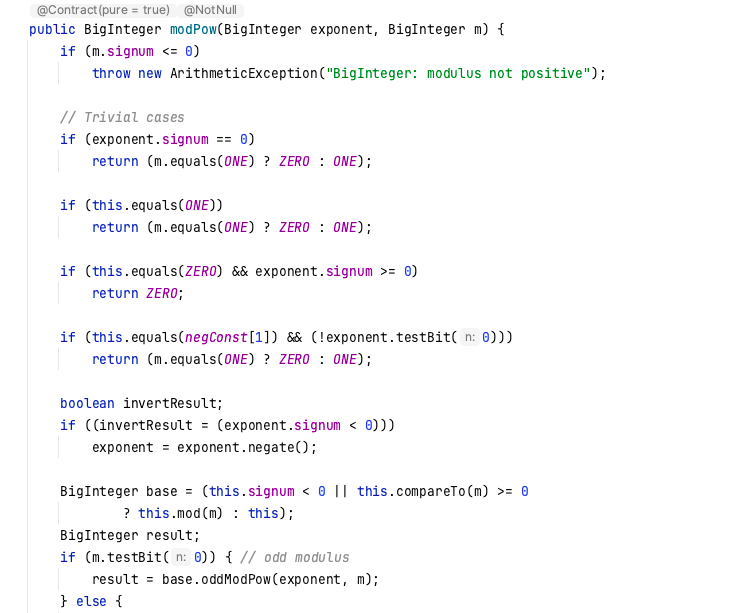
\includegraphics[scale = 0.5]{../IMAGES/Java/BigInt_modPow1.png}
     \label{fig_java_mPow3}
\end{figure}
\vspace{-1cm}
\begin{figure}[h]
     \centering
     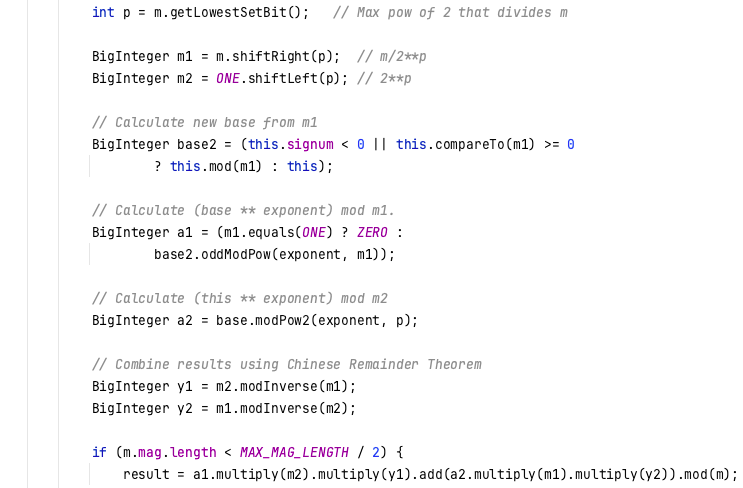
\includegraphics[scale = 0.5]{../IMAGES/Java/BigInt_modPow2.png}
     \label{fig_java_mPow4}
\end{figure}
\vspace{-1cm}
\begin{figure}[h]
     \centering
     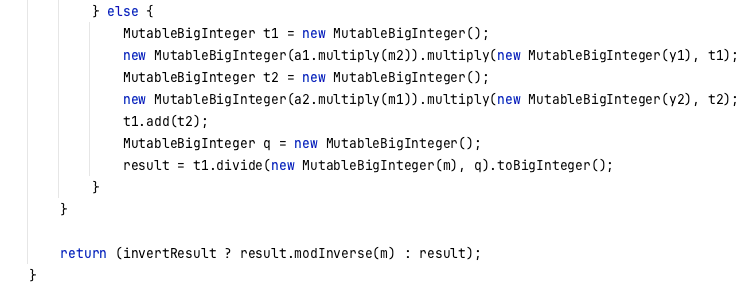
\includegraphics[scale = 0.5]{../IMAGES/Java/BigInt_modPow3.png}
     \caption{\large{Функція, яка використовується при піднесенні до степеня за mod.}}
     \label{fig_java_mPow5}
\end{figure}

\newpage
\uline{Метод \textbf{Java.math.BigInteger.modInverse()}} повертає модульну мультиплікативну інверсію this за mod m. Цей метод створює ArithmeticException, якщо $m <= 0$ або this не має мультиплікативного зворотного за модулем m (тобто $gcd(this, m) != 1$). 

\texttt{public BigInteger modInverse(BigInteger m)}

\uline{Параметри:} m -- модуль. 

\uline{Повернення:} метод повертає об’єкт BigInteger, значення якого дорівнює~$this^{-1}$ \textit{mod m}. 

\uline{Виняток:} ArithmeticException -- $m <= 0$, або цей BigInteger не має мультиплікативного зворотного за модулем m (тобто цей BigInteger не є взаємно простим до m).

\newpage
\uline{Приклад використання методу \textbf{BigInteger.Inverse()}:}

\begin{figure}[h]
     \centering
     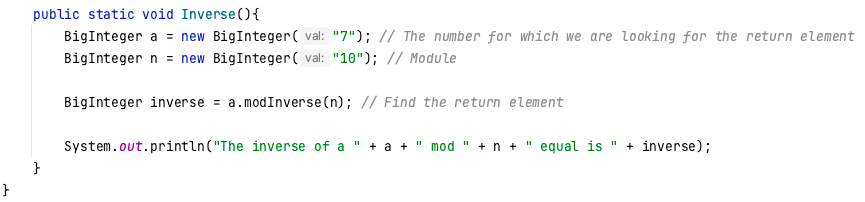
\includegraphics[scale = 0.49]{../IMAGES/Java/BigInt_Inv_ex.png}
     \caption{Приклад знаходження оберненого BigInteger за mod.}
     \label{fig_java_Inv1}
\end{figure}
\vspace{-1cm}
\begin{figure}[h]
     \centering
     
\includegraphics[scale = 0.5]{../IMAGES/Java/BigInt_Inv_output.png}
     \caption{Результат знаходження оберненого BigInteger за mod.}
     \label{fig_java_Inv2}
\end{figure}

\begin{figure}[h]
     \centering
     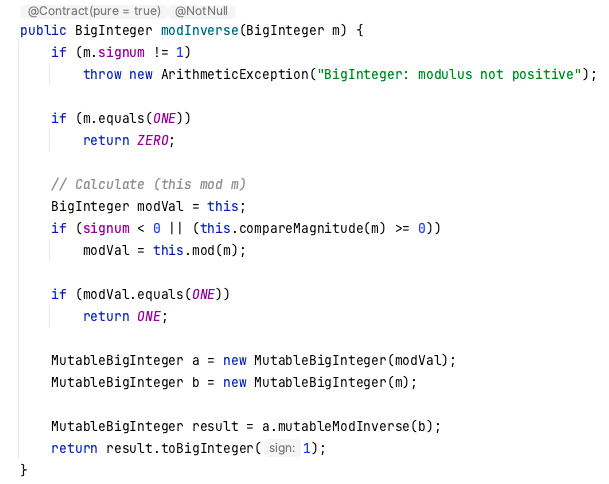
\includegraphics[scale = 0.49]{../IMAGES/Java/BigInt_Inv_doc.png}
     \caption{\large{Функція, яка використовується при знаходженні оберненого за mod.}}
     \label{fig_java_Inv3}
\end{figure}

\subsection{Використання GNU GMP бібліотеки у мові програмування Java}

\textbf{GNU GMP (GNU Multiple Precision Arithmetic Library)} -- це бібліотека на мові програмування C для виконання арифметики з довільною точністю. Щоб використовувати GMP в Java, можна скористатися JNI (Java Native Interface) або використовувати інші засоби для інтеграції коду на C в Java.

\uline{Операція піднесення до ступеня за модулем} за допомогою бібліотеки GNU GMP в Java використовує функцію \textit{'mpz powm'}. Також потрібно буде створити 2 файли -- GMPExample.java та GMPExample.c.

\uline{Приклад використання GMP в Java з допомогою JNI для піднесення числа до степеня за mod:}

\begin{figure}[h]
     \centering
     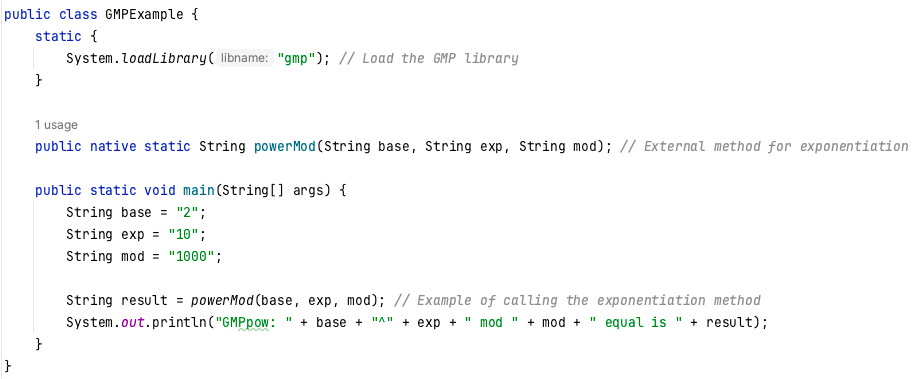
\includegraphics[scale = 0.5]{../IMAGES/Java/GMP_modPow_ex.png}
     \caption{Приклад коду у файлі GMPExample.java.}
     \label{fig_java_GMPpow_java}
\end{figure}

\begin{figure}[h]
     \centering
     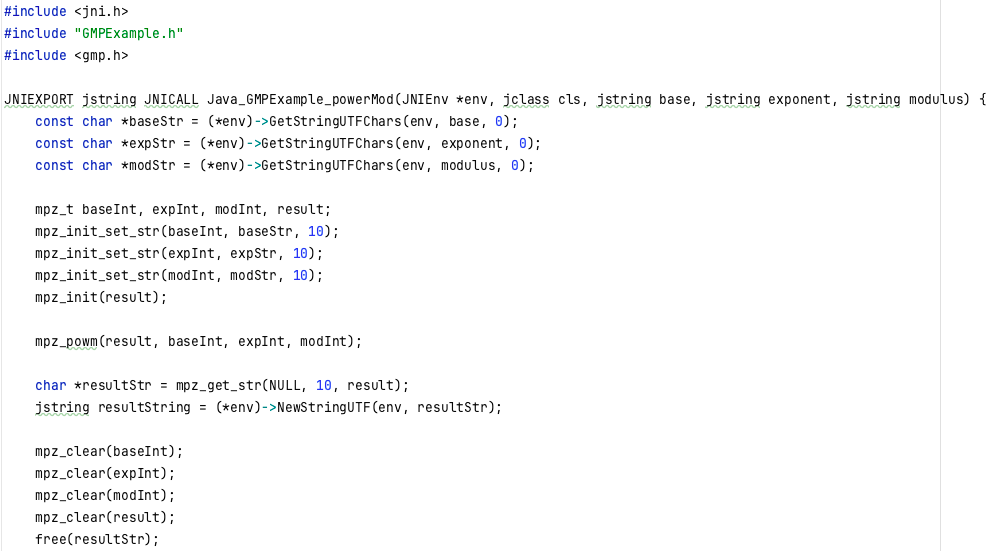
\includegraphics[scale = 0.5]{../IMAGES/Java/GMP_modPow_exC1.png}
     \label{fig_java_GMPpow_C1}
\end{figure}
\vspace{-1cm}
\begin{figure}[h]
     \centering
     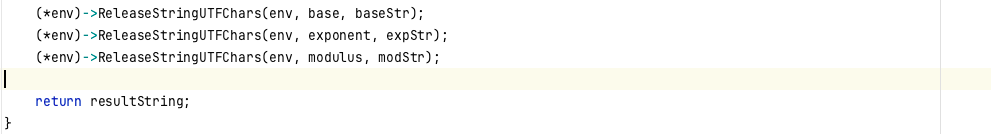
\includegraphics[scale = 0.5]{../IMAGES/Java/GMP_modPow_exC2.png}
     \caption{Приклад коду у файлі GMPExample.c.}
     \label{fig_java_GMPpow_C2}
\end{figure}

\newpage
Варто зазначити, що цей код треба компілювати з використанням gcc (GNU Compiler Collection) або іншого компілятора.

\vspace{10pt}
\uline{Операція інверсії (знаходження зворотного елемента)} для багаторозрядної арифметики в GNU GMP в Java використовує функцію \textit{'mpz invert'}. Ця функція знаходить обернений елемент по модулю, тобто, якщо c -- обернений елемент числа a за модулем b, то $a * c  \equiv 1 (mod b)$. 
Також потрібно буде створити 2 файли -- GMPExample.java та GMPExample.c.

\newpage
\uline{Приклад використання GMP в Java з допомогою JNI для знаходження зворотного числа за mod:}

\begin{figure}[h]
     \centering
     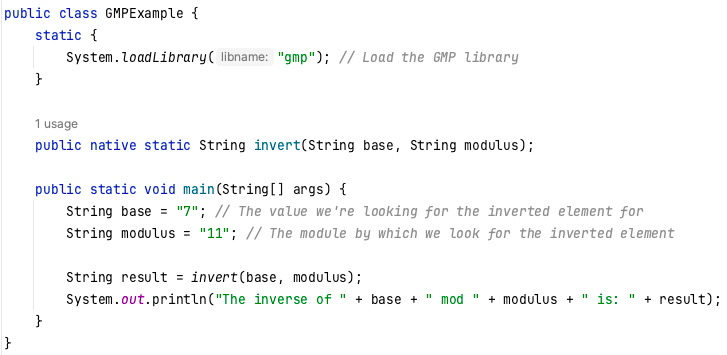
\includegraphics[scale = 0.35]{../IMAGES/Java/GMP_inv_exJava.png}
     \caption{Приклад коду у файлі GMPExample.java.}
     \label{fig_java_GMPinv_java}
\end{figure}
\vspace{-1cm}
\begin{figure}[h]
     \centering
     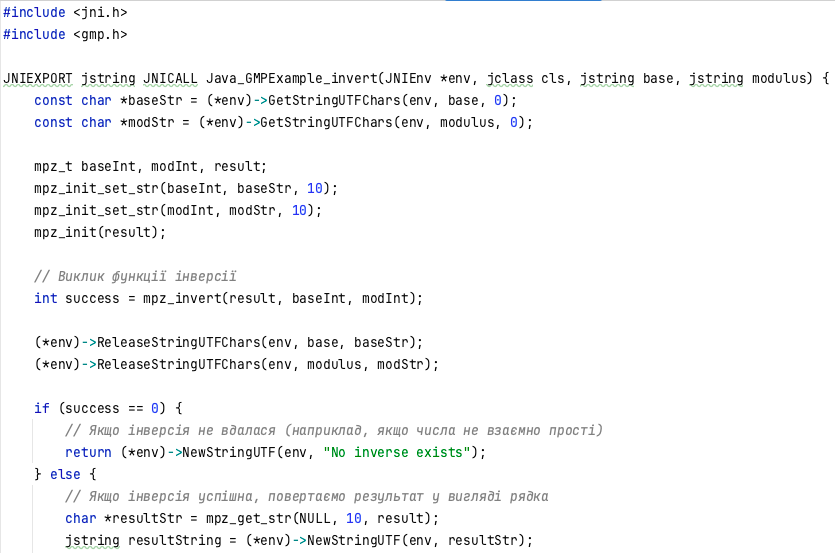
\includegraphics[scale = 0.37]{../IMAGES/Java/GMP_inv_exC1.png}
     \label{fig_java_GMPinv_C1}
\end{figure}
\vspace{-1cm}
\begin{figure}[h]
     \centering
     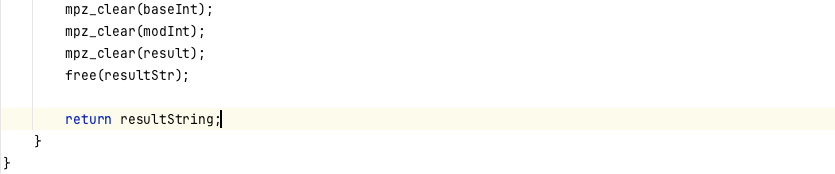
\includegraphics[scale = 0.37]{../IMAGES/Java/GMP_inv_exC2.png}
     \caption{Приклад коду у файлі GMPExample.c.}
     \label{fig_java_GMPinv_C2}
\end{figure}

Обернений елемент числа a за модулем b існує, якщо a і b взаємно прості.

\subsection{Висновки до розділу Java}

Мова програмування Java є високофункціональною та гнучкою для роботи з багаторозрядною арифметикою. Вбудована бібліотека BigInteger надає зручний інтерфейс для операцій над дуже великими цілими числами, забезпечуючи високу точність без втрати продуктивності.

Крім цього,існує можливість використання сторонніх обгорток та інтерфейсів, таких як Java GMP (jGMP) та Java MPFR (jMPFR) для бібліотек GMP (GNU Multiple Precision Arithmetic Library) та MPFR (Multiple Precision Floating-Point Reliable Library) відповідно. Оскільки завдяки ним розширюються можливості Java у сфері багаторозрядної арифметики. Використання цих обгорток дозволяє розробникам Java використовувати потужні функціональності GMP та MPFR у своїх проектах, розширюючи можливості багаторозрядної арифметики та операцій з плаваючою комою в Java.

Усі ці можливості дають розробникам можливість обирати інструмент, який найкраще відповідає конкретним вимогам їх проекту. Зручний інтерфейс BigInteger та висока продуктивність сторонніх бібліотек роблять Java ефективним інструментом для вирішення різноманітних математичних завдань у світі програмування.

% Створюємо висновки
\conclusions
\input{../CHAPTERS/w1_conclusions}

% Додаємо бібліографію
% Якщо ви володієте магією bibtex-у, використовуйте її та модифікуйте файл 
% з бібліографією відповідним чином
%\bibliographylist
%\printbibliography[heading=none]

% Створюємо додатки (дивись у файли додатків для необхідних пояснень)
% Якщо ви маєте меншу або більшу кількість додатків, модифікуйте наступні 
% рядки відповідним чином
% Якщо ви не маєте додатків, просто закоментуйте наступні рядки
%\input{../CHAPTERS/z1_appendix_A}


% Нарешті
\end{document}